%%%%%%%%%%%%%%%%%%%%%%%%%%%%%%%%%%%%%%%%%
% Short Sectioned Assignment
% LaTeX Template
% Version 1.0 (5/5/12)
%
% This template has been downloaded from:
% http://www.LaTeXTemplates.com
%
% Original author:
% Frits Wenneker (http://www.howtotex.com)
%
% License:
% CC BY-NC-SA 3.0 (http://creativecommons.org/licenses/by-nc-sa/3.0/)
%
%%%%%%%%%%%%%%%%%%%%%%%%%%%%%%%%%%%%%%%%%

%------------------------------------------------------------------------
%PACKAGES AND OTHER DOCUMENT CONFIGURATIONS
%------------------------------------------------------------------------

\documentclass[paper=a4, fontsize=11pt]{report} % A4 paper and 11pt font size
\usepackage[swedish, english]{babel}            % Swedish and English language/hyphenation
\usepackage[T1]{fontenc}                        % use 8-bit encoding that has 256 glyphs
\usepackage[a4paper]{geometry}
\usepackage{hyperref}
\usepackage[myheadings]{fullpage}
\usepackage{fancyhdr}
\usepackage{lastpage}
\usepackage{graphicx, wrapfig, subcaption, setspace, booktabs}
\usepackage[T1]{fontenc}
\usepackage[font=small, labelfont=bf]{caption}
\usepackage{fourier}
\usepackage[protrusion=true, expansion=true]{microtype}
\usepackage{sectsty}
\usepackage{url, lipsum}
\usepackage{amsmath}
\usepackage{float}
\usepackage{lmodern}
\usepackage[normalem]{ulem}
\useunder{\uline}{\ul}{}

%------------------------------------------------------------------------
%TITLE SECTION
%------------------------------------------------------------------------

\newcommand{\horrule}[1]{\rule{\linewidth}{#1}}       % Create horizontal rule command with 1 argument of height
\onehalfspacing
\setcounter{tocdepth}{5}
\setcounter{secnumdepth}{5}
\usepackage{titlesec}
%
\pagestyle{fancy}
\fancyhf{}
\setlength\headheight{15pt}
\fancyhead[L]{Niklas Eliasson, Victor Persson}
\fancyhead[R]{Luleå Tekniska Universitet}
\fancyfoot[C]{\thepage}
%
\begin{document}
%
\title{
	\normalfont \normalsize
	\textsc{Luleå Tekniska Universitet} \\ [25pt] % Your university, school and/or department name(s)
	\horrule{1pt} \\[0.4cm]                       % top horizontal rule
	\huge Sprint 4 \\                             % The assignment title
	\horrule{1pt} \\[0.5cm]                       % bottom horizontal rule
}
%
\author{Victor Persson,\\ Niklas Eliason}             % Your name
%
\date{\normalsize\today}                              % Today's date or a custom date
%
\maketitle                                            % Print the title
%
\tableofcontents
\thispagestyle{empty}
\sectionfont{\scshape}
%
\newpage
\setcounter{page}{1}

%------------------------------------------------

\section*{Summary}
\addcontentsline{toc}{section}{Summary}
	We are working on a e-commerce site for selling patches and accessories such as
	belts and zippers for student overalls. It is intended to be dynamic with a
	fully functional content management system. \\
	For educational purposes Ruby on Rails was chosen. \\
	Scrum planing was done at Trello.com and GitHub.com was used as VCS. \\

	User stories was set up to define what functionality we wanted the site
	to have. From this the database schema was defined. The user
	stories were then broken down into Scrum stories and tasks, given importance
	and time estimates. Some basic test cases were added.

	The biggest challenges were were time-estimates and scope-creep.

	We decided not to try to implement any payment methods. Sales campaigns,
	though drafted, were later dropped.

\section*{Methodology}
\addcontentsline{toc}{section}{Methodology}

	First a quick mock-up was done. From this user stories was drafted to see what kind of functionality should be included. The functionality were translated to the first draft of a database schema by identifying all nouns and writing them on Post-Its. Every noun became an entity, a table, and was given properties. Relationships were mapped and where there was a many to many relationship connecting tables were added.

	The user stories were then broken down into backlog stories, which were further broken down into tasks. Every story was given an importance rating and a time estimate. New, improved design mock-ups were drafted for frontend-oriented stories.

	Halfway through each sprint the sprint backlog was reviewed and stories were re-prioritized and re-estimated. After each sprint a sprint-review was held, and before every sprint started a sprint planning meeting was held, reworking the product backlog and adding tasks that had come up during the preceding sprint.

\section*{User stories}
\addcontentsline{toc}{section}{User stories}

	\subsection*{Register an account}
	\addcontentsline{toc}{subsection}{Register}
	\begin{enumerate}
		\item User arrives at the page. Figure \ref{fig:start}
		\item An unregistered user can only browse the site if the user tries to use any functionality he will be taken to the login page which will let him register. Figure \ref{fig:login}
		\item User provides minimal amount of info needed for an account. Figure \ref{fig:register}
		\item On successful registration the user is greeted with a message and can now start using the site fully. Figure \ref{fig:register_done}
	\end{enumerate}


	\subsection*{Edit profile}
	\addcontentsline{toc}{subsection}{Edit profile}
	\begin{enumerate}
		\item By pressing the "Profil" button in the menu the user can access his profile. User sees that his full profile isn't filled in, so he presses "Ändra" (change). Figure \ref{fig:profile}
		\item This brings the user to the profile editing page, where he can fill in the rest of his information. Figure \ref{fig:edit_profile}
	\end{enumerate}


	\subsection*{Place order}
	\addcontentsline{toc}{subsection}{Place order}
	\begin{enumerate}
		\item The user browses the categories and finds something he likes, in this case patches. He does not, however know what kind of patches he's interested in so he presses patches, which renders all products of the subcategories as well. Figure \ref{fig:products}
		\item The user finds a product he likes and can either add it to his cart directly or click the product and be brought to the product page, containing more information.
		\item In this case he wants to know a little more about the product. He's taken to the product page where he can read some more info, see the rating of the product or read reviews from other users. Figure \ref{fig:product}
		\item After browsing for a while and adding some products it's time to check out. He clicks "Kundkorg" to review his cart. Figure \ref{fig:cart}
		\item After checking that everything is correct he presses "Kassa" and is taken to the checkout
		\item To place an order an address has to be given. Since this user has filled in his full profile information his address is sourced from the profile, but could be changes by the user if he wishes this order to be delivered somewhere else. \ref{fig:order}
		\item Upon completion the user is greeted with a success message and an order confirmation. Figure \ref{fig:order_confirmation}
	\end{enumerate}


	\subsection*{Adding a review}
	\addcontentsline{toc}{subsection}{Adding a review}
	\begin{enumerate}
		\item The user has received his products and now wishes to add a review to it.
		\item He goes to the product he ordered. \ref{fig:comments}
		\item Here he can either leave just a rating, or as in this case add a review. He cannot, however leave a review without giving a rating.
		\item Upon completion he is greeted with a success message and can control that the review is correct.
		\item If, in the future, the user would change his mind about the product he can go back and either change or remove the review. \ref{fig:comment_added}
	\end{enumerate}


	\subsection*{Changing something as an admin}
	\addcontentsline{toc}{subsection}{Changing something as an admin}
	\begin{enumerate}
		\item An admin signs in just as a regular user. Figure \ref{fig:login}
		\item After signing in the admin is greeted with some changes in the interface for a more streamlined experience for changing things. Figure \ref{fig:admin}
	\end{enumerate}



\section*{User roles}
\addcontentsline{toc}{section}{User roles}

% TODO: translate to Eng
% TODO: make sure user roles are correct
% TODO: add non logged-in users
% TODO? maybe change to table in following (should be easy with Vim-macro) form:
%
%  Store owner
%  ---------------------------------
% | Read | Write |             Item |
% |---------------------------------|
% |    x |     x |         Products |
% |    x |       | Customer profile |
%  ---------------------------------

Användare
\begin{itemize}
	\item Butiksadministratör
		\begin{itemize}
			\item r/w priser
			\item r/w kampanjer
			\item r/w lagerstatus
			\item r/w kategorier
			\item r/w reviews (for cleaning up spam)
			\item r leveransstatus
			\item r kundinfo
		\end{itemize}
	\item Lagerarbetare
		\begin{itemize}
			\item r/w lagerstatus
			\item r/w leveransstatus
			\item r kundinfo
		\end{itemize}
	\item Inloggad kund
		\begin{itemize}
			\item r/w sin egen kontaktinformation
			\item r/w own reviews
			\item r other customers reviews
			\item läsa sin egen orderhistorik
			\item läsa sortimentet (produkter, priser, kampanjer, lagerstatus)
			\item lägga ordrar
			\item Spara/skicka kundkorg
		\end{itemize}
	\end{itemize}

	See Figure \ref{fig:2} - \ref{fig:4}

	\begin{figure}
		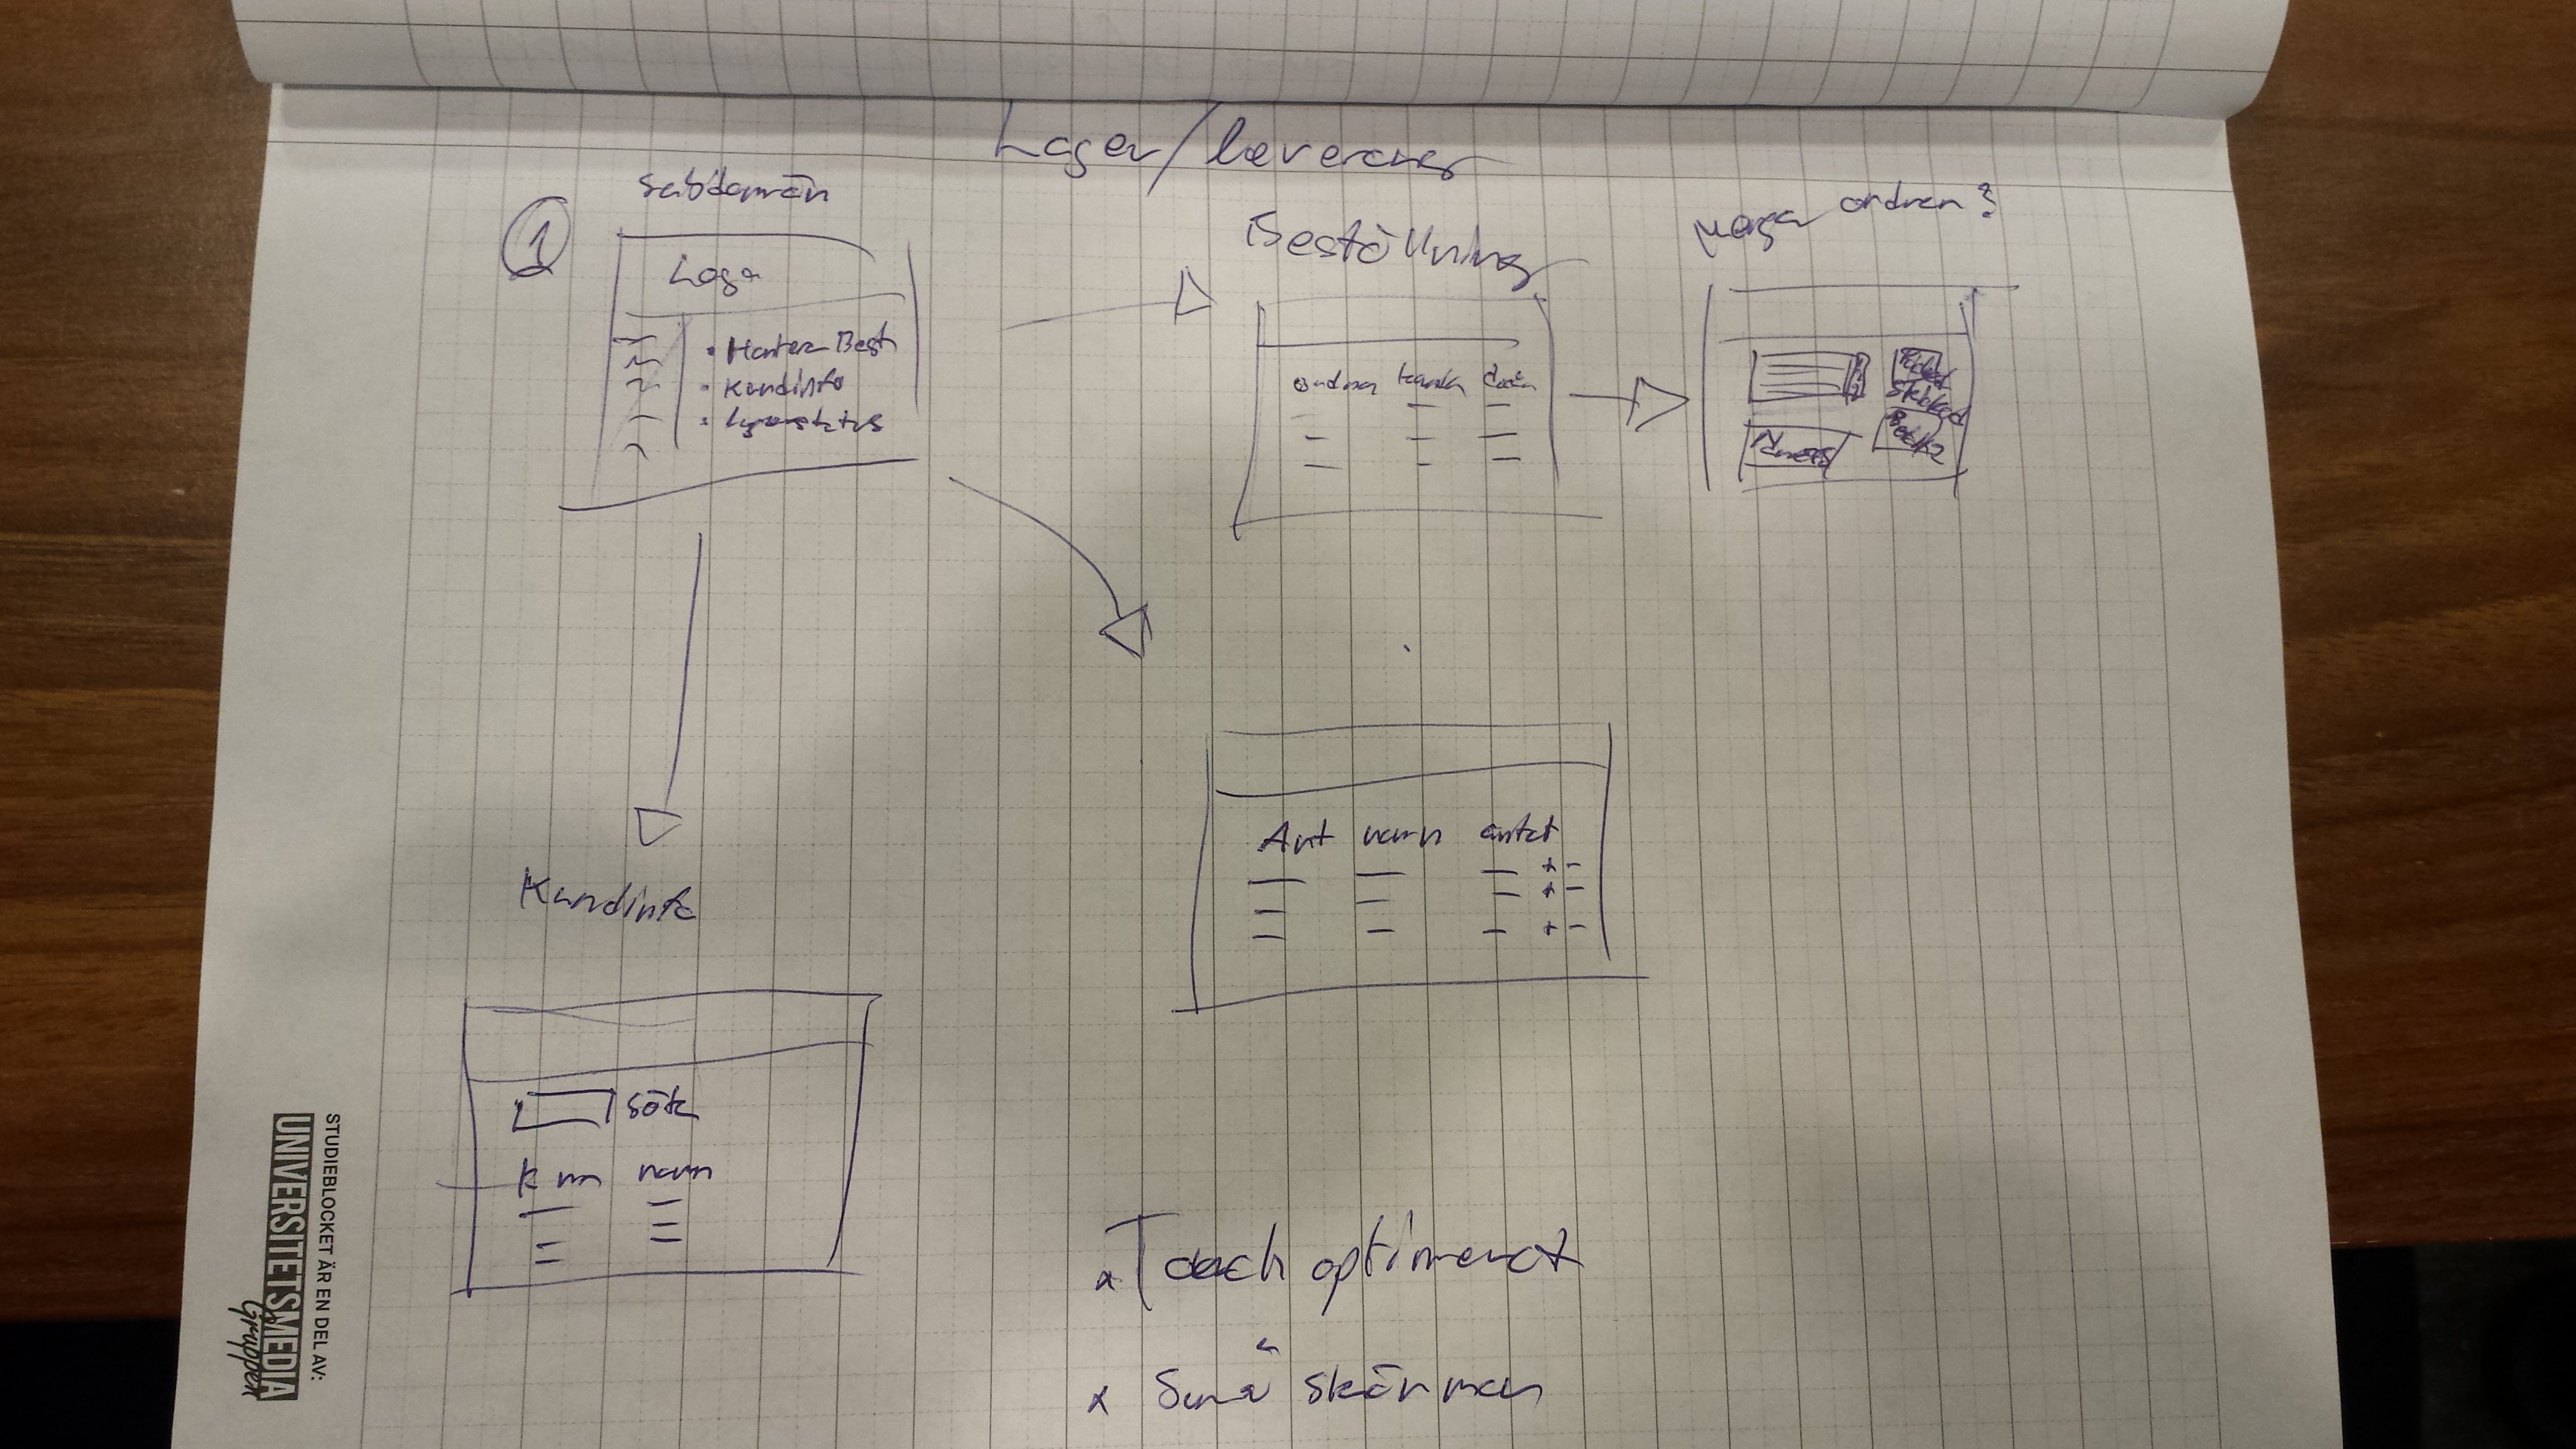
\includegraphics[scale=0.12]{artifacts/Lager.jpeg}
		\caption{}
		\label{fig:2}
	\end{figure}

	\begin{figure}
		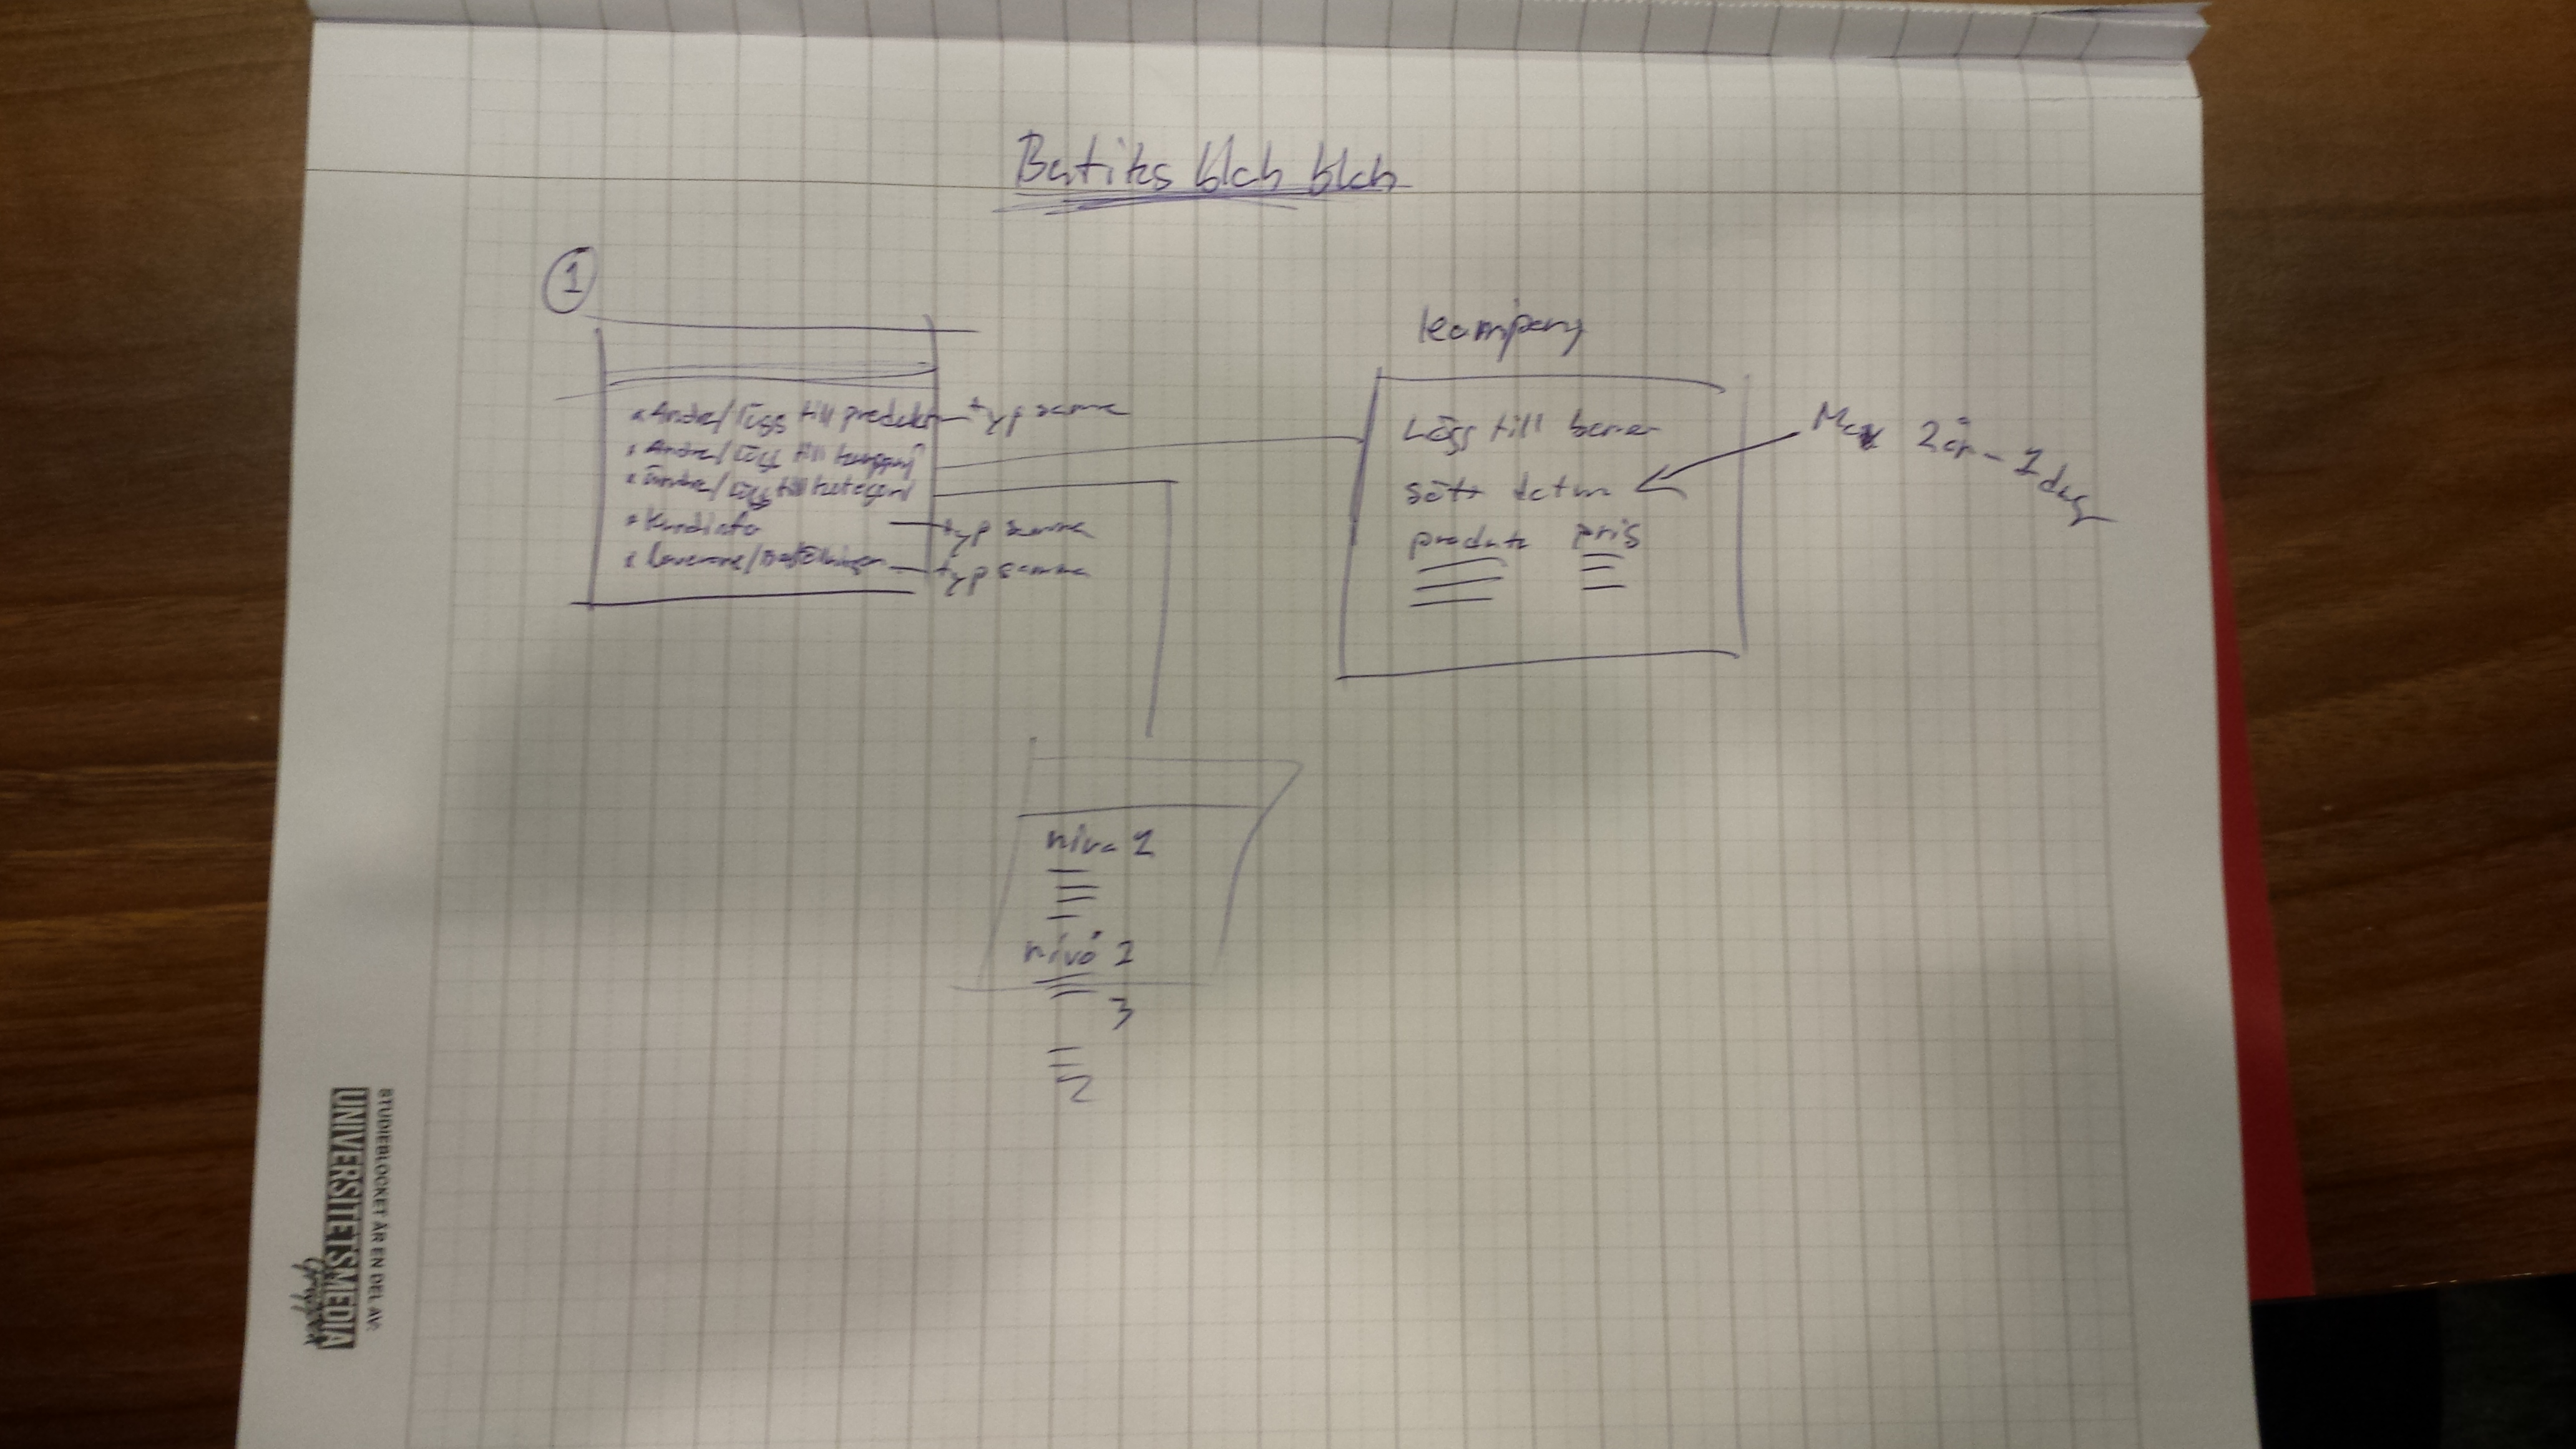
\includegraphics[scale=0.12]{artifacts/ButiksAdmin.jpeg}
		\caption{}
		\label{fig:3}
	\end{figure}

	\begin{figure}
		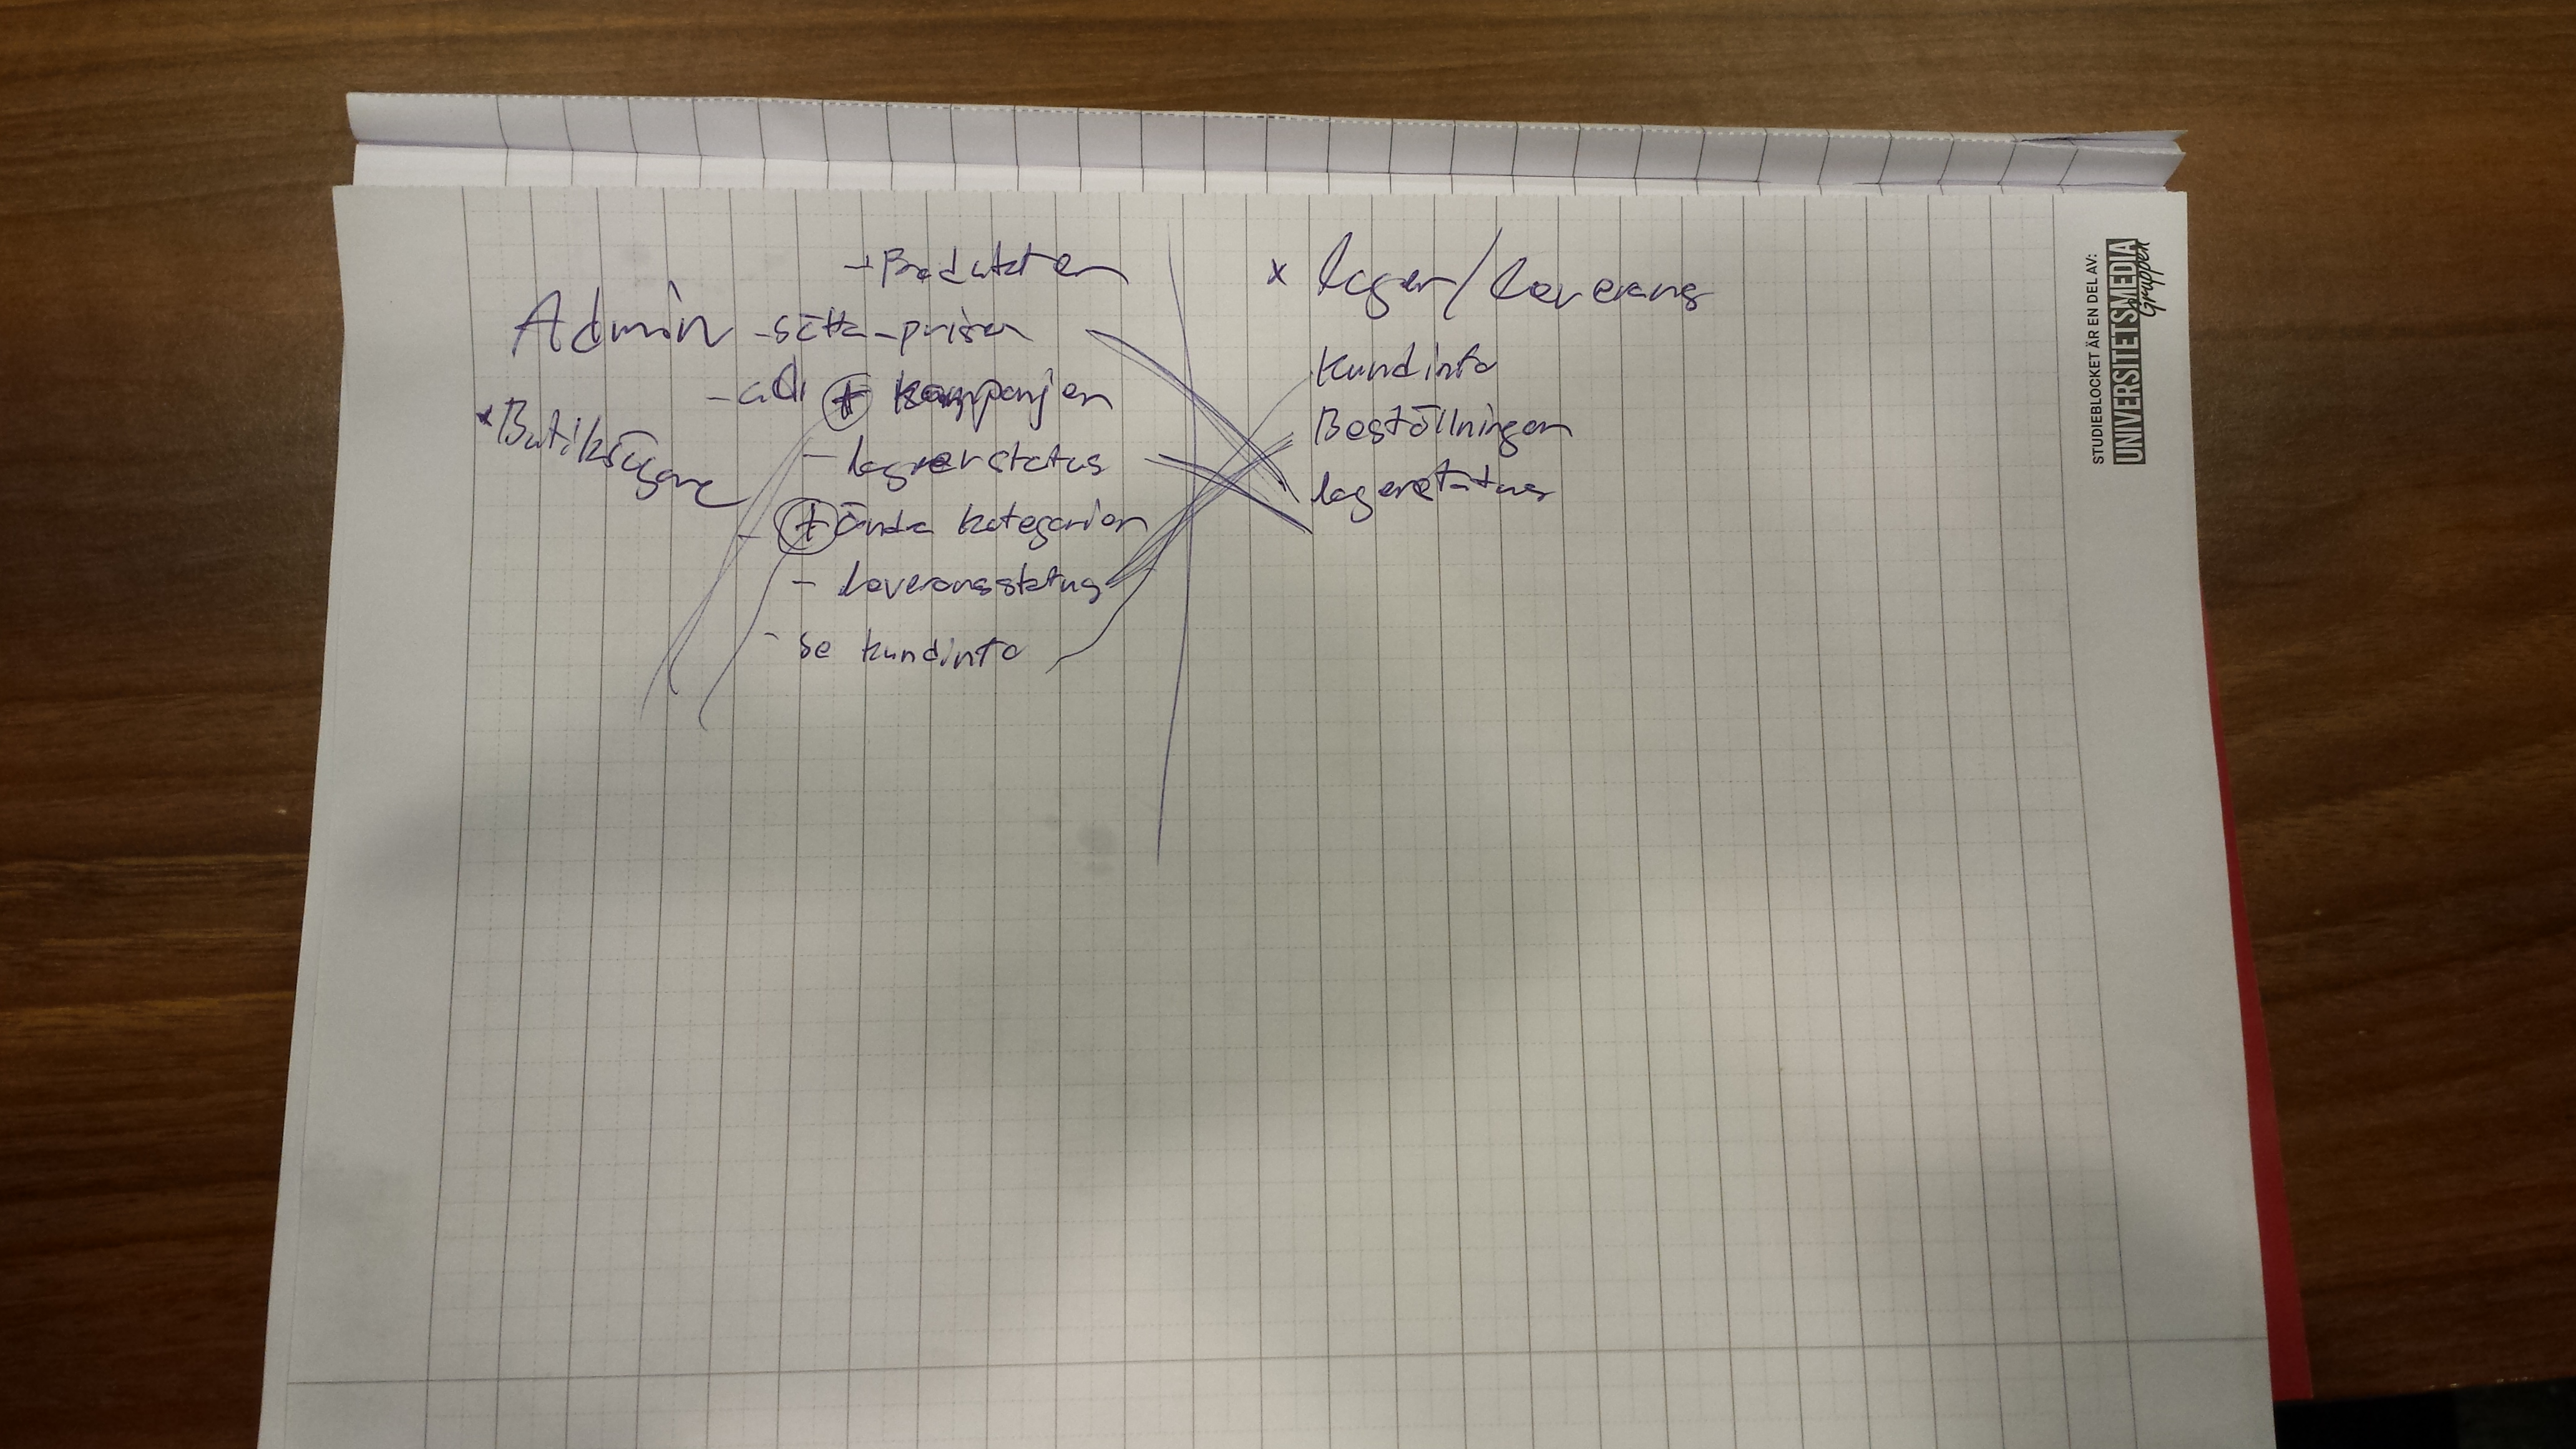
\includegraphics[scale=0.12]{artifacts/Admin.jpeg}
		\caption{}
		\label{fig:4}
	\end{figure}

\section*{System architecture}
\addcontentsline{toc}{section}{System architecture}
	During development we run the system on Ruby on Rails' (RoR) built in web server
	Puma and SQLight3 for simplicity, but intend to move to a MariaDB database
	and a Nginx web server with Phusion Passenger for RoR. We host
	the servers ourselves because it seemed seemed fun, educational and fairly simple.

\section*{Backlog}
\addcontentsline{toc}{section}{Backlog}

	The backlog was made after discussions after breaking down the user stories
	into backlog stories, which were further broken down into tasks. They were
	then given priorities and time estimates. We tried to have a sit down halfway
	through every sprint to see if any stories needed to be broken down into
	smaller stories or if some stories needed to be combined. After that the
	stories would be re-prioritized and re-estimated.

	These backlog items were dealt with during this (last) sprint.
	Figure \ref{fig:trello_final} includes a snapshot of the scrum board
	at the end of this sprint. \\

	\begin{tabular}{|l|l|l|l|}
		\hline
		\#  & Sprint 4                      & Priority & Time est. \\ \hline
		301 & Startsida                     & 100      & 2         \\ \hline
		302 & Dynamisk meny från kategorier & 90       & 2         \\ \hline
		304 & Produktsida                   & 110      & 4         \\ \hline
		305 & Kundkorg                      & 80       & 8         \\ \hline
		307 & Profilsida (kundkort)         & 45       & 2         \\ \hline
		308 & Orderhistorik                 & 45       & 1         \\ \hline
		309 & Kundinlogg                    & 50       & 2         \\ \hline
		310 & Registrering                  & 60       & 4         \\ \hline
		312 & kommentarer/betygsättning     & 70       & 8         \\ \hline
		313 & Produktkategorier             & 75       & 2         \\ \hline
		400 & Backendinloggning             & 25       & 2         \\ \hline
		1   & Personnummer -/+ hantering    & 5        & 1         \\ \hline
	\end{tabular} \\


	These stories were put on hold and eventually scrapped from the project.

	\begin{tabular}{|l|l|l|l|}
		\hline
		\#  & Left in backlog  & Priority & Time est. \\ \hline
		410 & Kampanjhantering & 10       & 3         \\ \hline
		311 & Produktsökning   & 45       & 1         \\ \hline
		306 & Betalsida        & 5        & 12        \\ \hline
	\end{tabular}

	Planing is done at Trello.com
	\url{https://trello.com/b/JxDCHBcm} \\
	This is just a small section of the backlog. For history of all sprints and deeper
	explanation of the backlog items, refer to Trello.


	\begin{figure}[h]
		\includegraphics[width=\textwidth]{artifacts/trello_sprint1.png}
		\caption{Screenshot of the scrum board going into the second sprint.}
		\label{fig:trello_sprint1}
	\end{figure}

	\begin{figure}[h]
		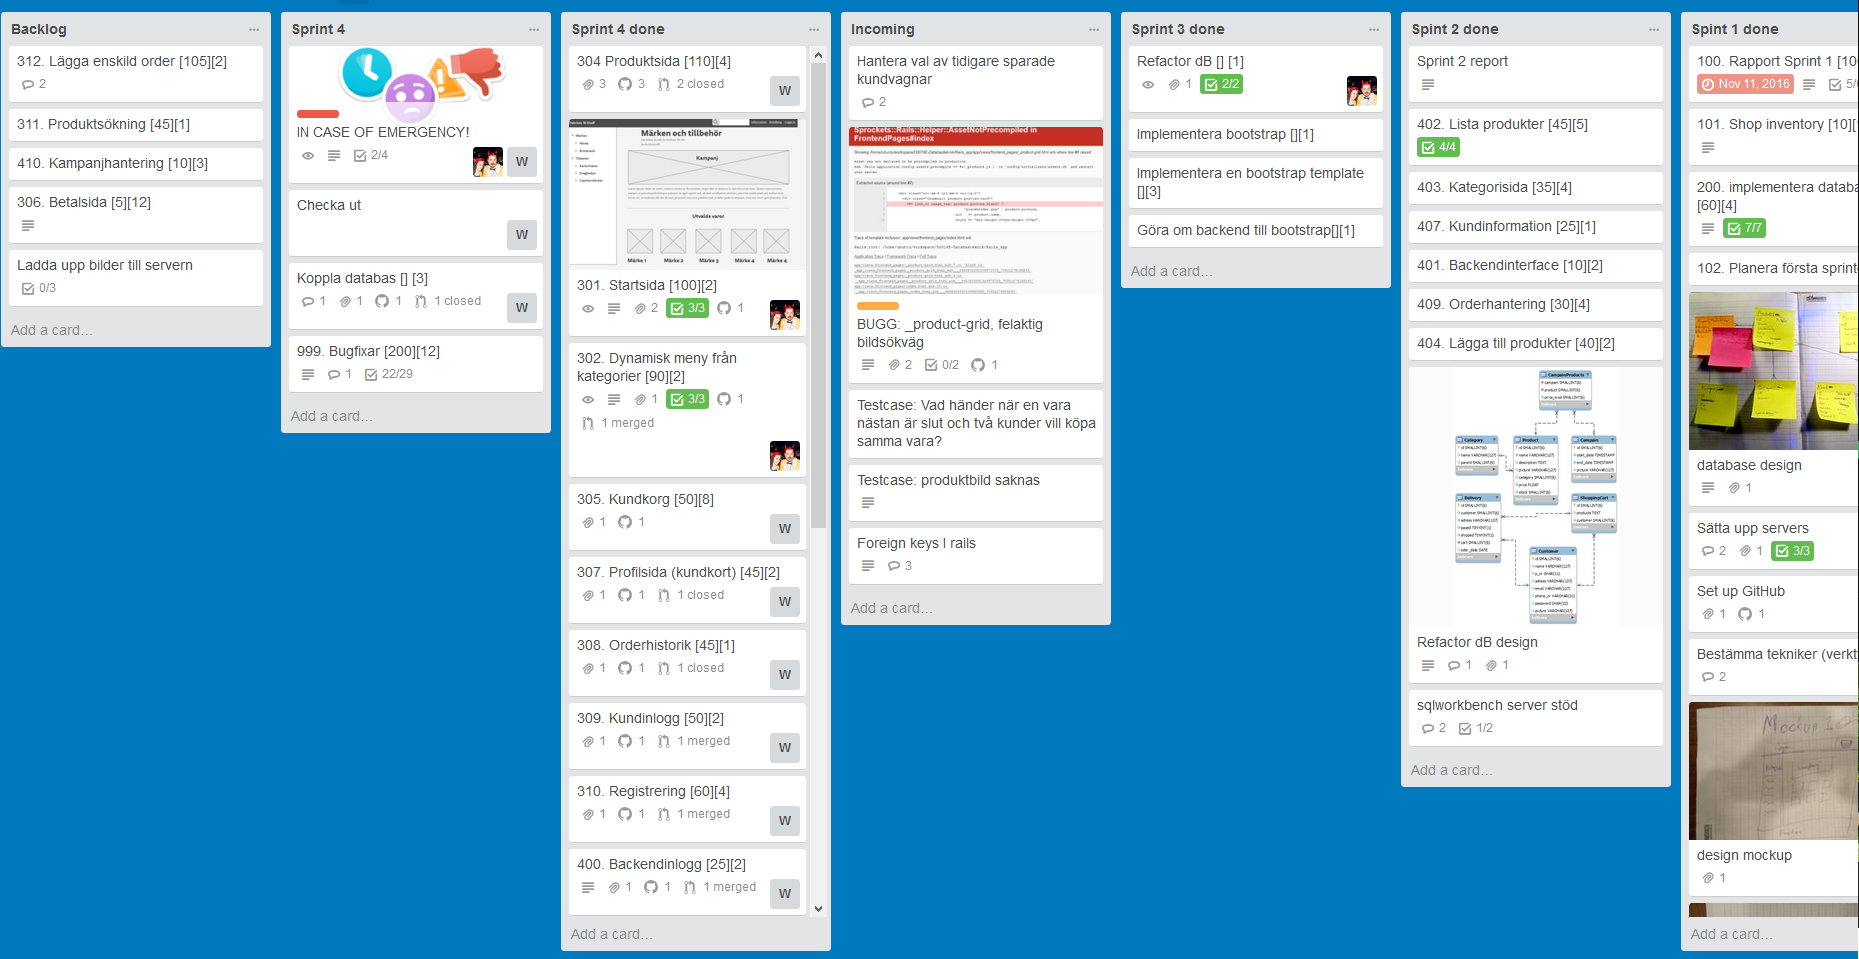
\includegraphics[width=\textwidth]{artifacts/trello_final.png}
		\caption{Screenshot of the current state of the scrum board.}
		\label{fig:trello_final}
	\end{figure}

\section*{Database schema}
\addcontentsline{toc}{section}{Database schema}
See Figure \ref{fig:db}

\begin{figure}
	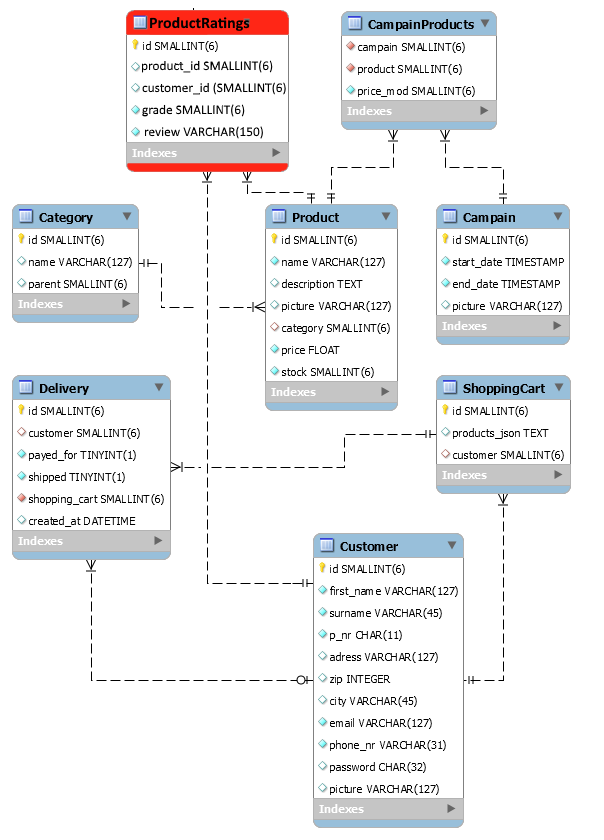
\includegraphics[width=\textwidth]{artifacts/db_implemented_1_3.png}
	\caption{Database design. (not including reworked ShoppingCart)}
	\label{fig:db}
\end{figure}

\section*{Code}
\addcontentsline{toc}{section}{Code}
All code is available at github.
\url{https://github.com/nikalas/D0018E-Databasteknik.git}

\section*{Test case specifications}
\addcontentsline{toc}{section}{Test case specifications}

% TODO? Did we define more test cases?
% TODO: Should include some unit tests.

	Problem: Item out of stock? \\
		A customer adds a product to the basket. If the product goes out of
		stock before checkout, how is this handled?

	Solution: \\
		At checkout a check is made if all the products in the shoppign cart 
        is in stock. If not the customer is brought back to the "carts" page 
        and asked to remove the product(s) that is no longer available and
        that the cart has to be updated.

\section*{Limitations and improvements}
\addcontentsline{toc}{section}{Limitations and improvements}

	We decided to put off saving payment methods and/or information. Might
	end up re-adding it to the backlog if it looks like we will have time
	to spare. Non-registered customers have also pretty much been put on hold for now.
	Products search, sorting, sale campaigns, and uploading pictures
	through the backend has also been put on hold, since we didn't have
	time to fully implement them. In a few places the internal quality is suffering and
	some refactoring could most certainly benefit the code.

\section*{Challenges and problems}
\addcontentsline{toc}{section}{Challenges and problems}

	The greatest challenges were no doubt time estimates and scope-creep. As you learn more, you want to add more, risking not making the deadline and letting other features fall behind. Another problem we had was that RoR's ActiveRecord does a whole lot for you. This means that you can set everything up really good in the rails models, but the actual database isn't very well optimized.
	Another problem we had was that even though there are some unit tests in place, it's easy to forget to do manual testing. When you're working on a deadline this makes quite some bugs slip through which resulted in us having to spend the entire last 24 hours before hand-in with testing and bugfixing. And there were a few (see figure \ref{fig:bugs}). We did manage to get them down from 28 to 6, most remaining being purely superficial though.
	All in all thought we didn't really have any big problems. Probably because  we did a lot of structured planning going into the project.

\begin{figure}
	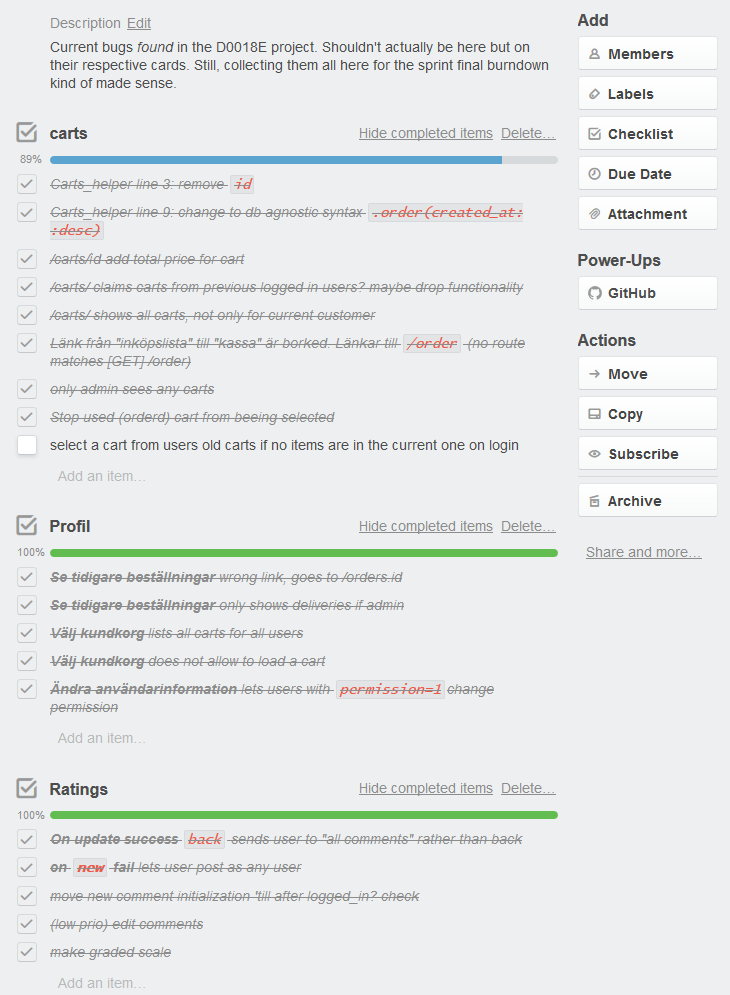
\includegraphics{artifacts/bugs}
	\caption{A few of the last-minute bugs.}
	\label{fig:bugs}
\end{figure}

%-------- User story Images -------

\begin{figure}
	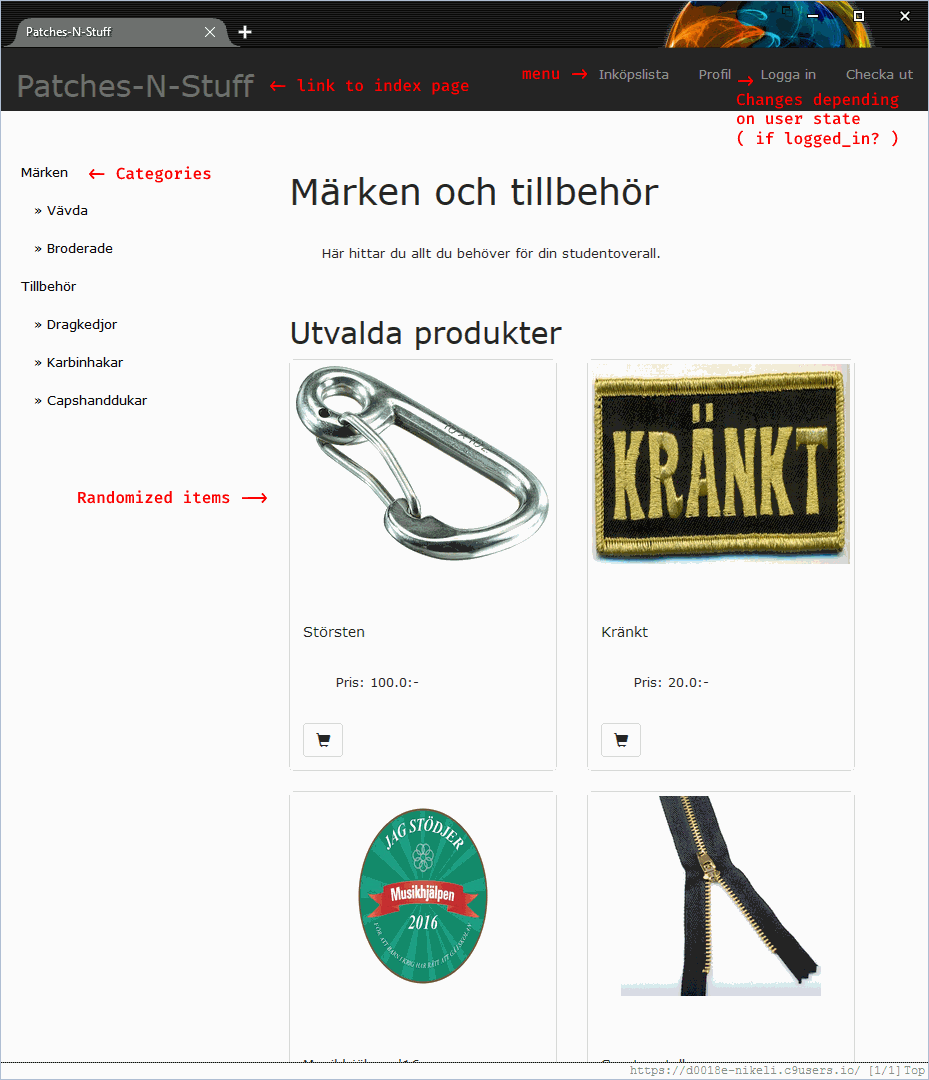
\includegraphics[width=0.9\paperwidth]{artifacts/stories/1_start.png}
	\caption{Greeting page of the web shop.}
	\label{fig:start}
\end{figure}

\begin{figure}
	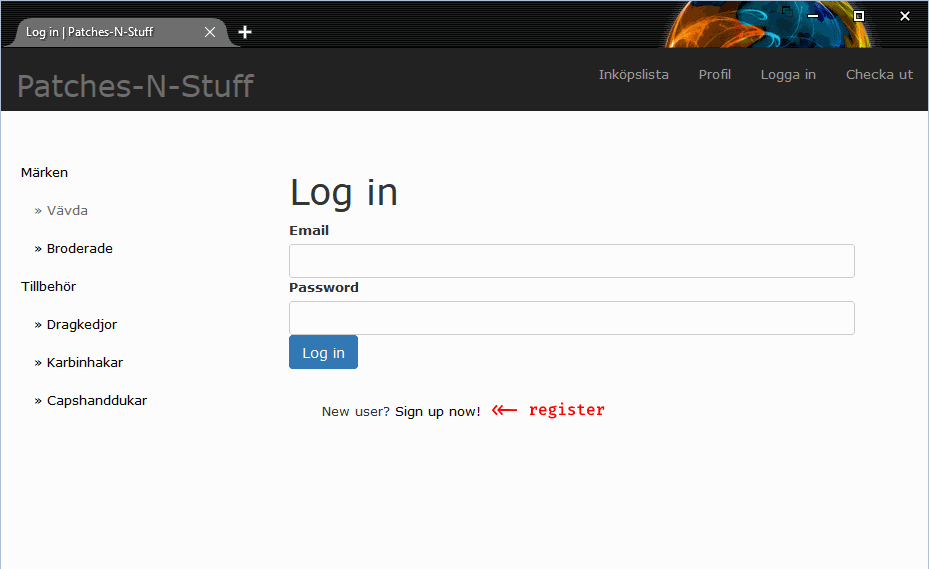
\includegraphics[width=0.9\paperwidth]{artifacts/stories/2_login.png}
	\caption{Login page}
	\label{fig:login}
\end{figure}

\begin{figure}
	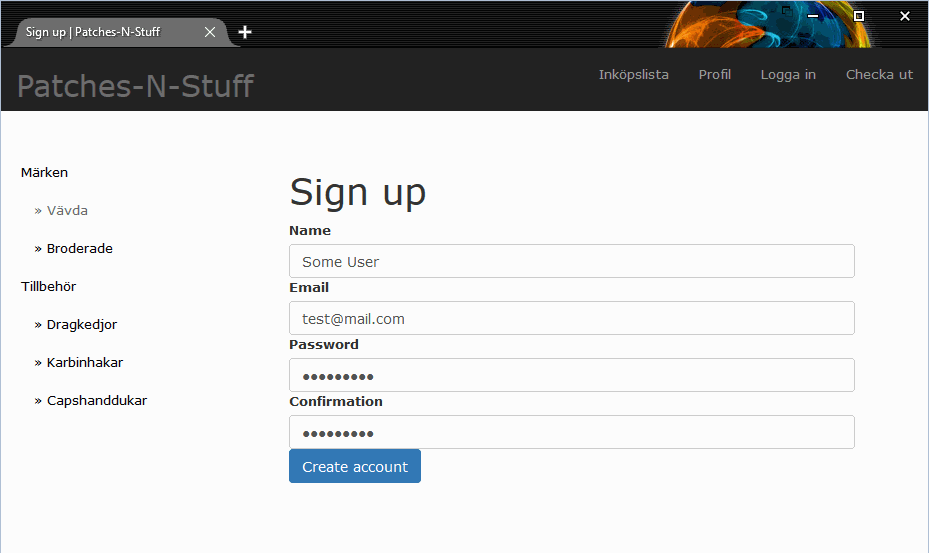
\includegraphics[width=0.9\paperwidth]{artifacts/stories/3_register.png}
	\caption{Register page}
	\label{fig:register}
\end{figure}

\begin{figure}
	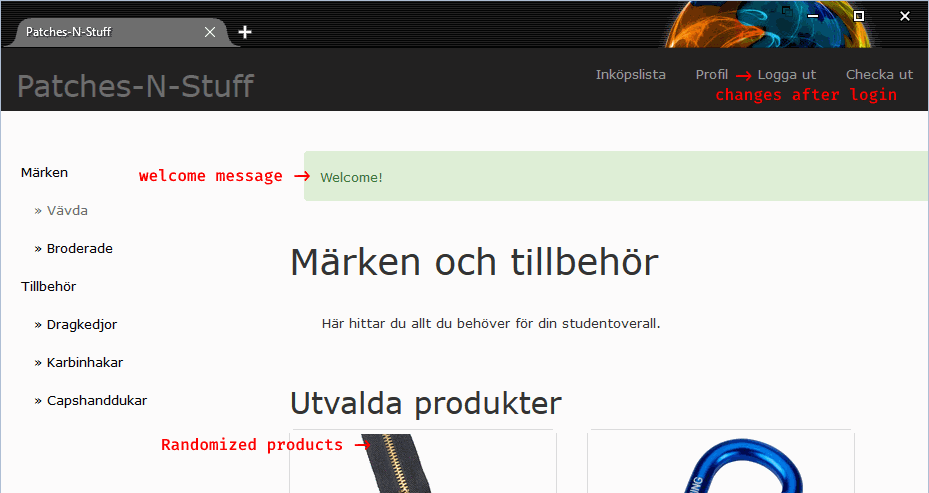
\includegraphics[width=0.9\paperwidth]{artifacts/stories/4_register_done.png}
	\caption{Registration complete}
	\label{fig:register_done}
\end{figure}

\begin{figure}
	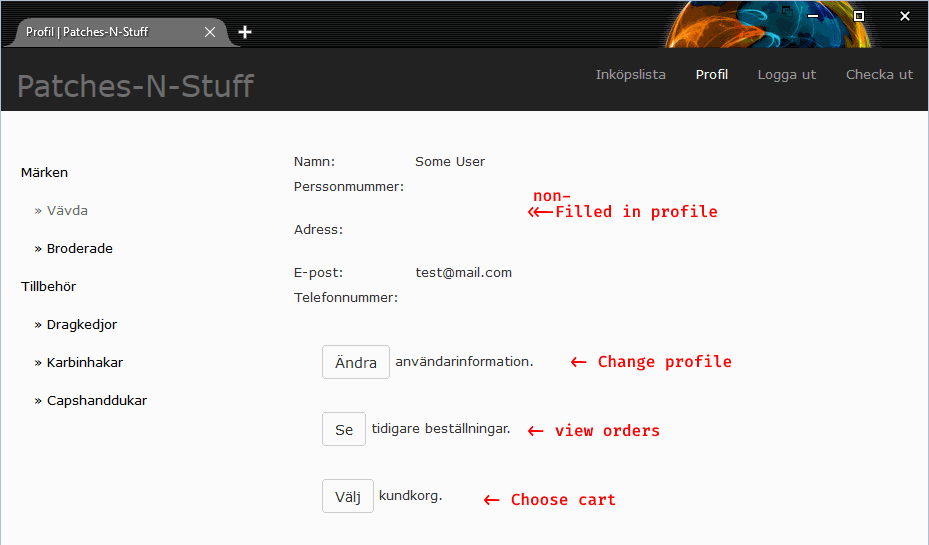
\includegraphics[width=0.9\paperwidth]{artifacts/stories/5_profile.png}
	\caption{Profile page}
	\label{fig:profile}
\end{figure}

\begin{figure}
	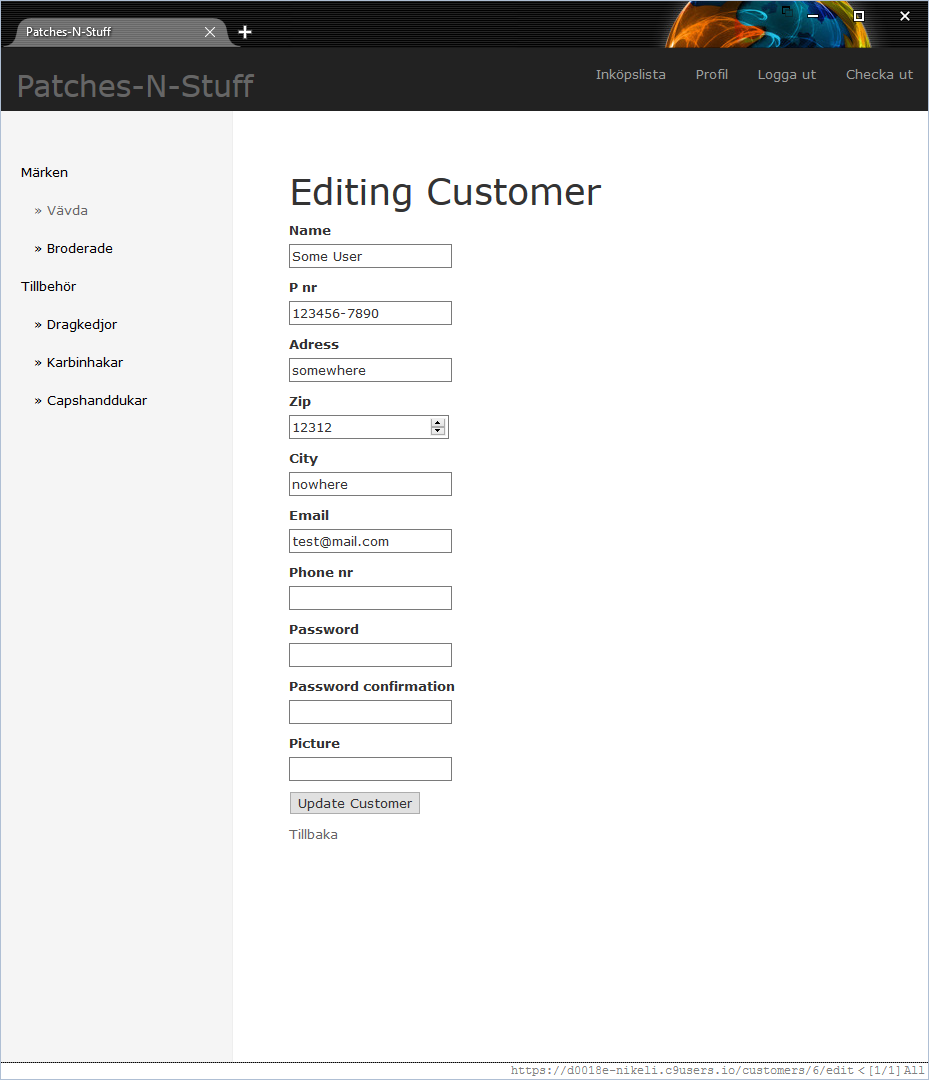
\includegraphics[width=0.9\paperwidth]{artifacts/stories/6_edit_profile.png}
	\caption{Edit profile}
	\label{fig:edit_profile}
\end{figure}

\begin{figure}
	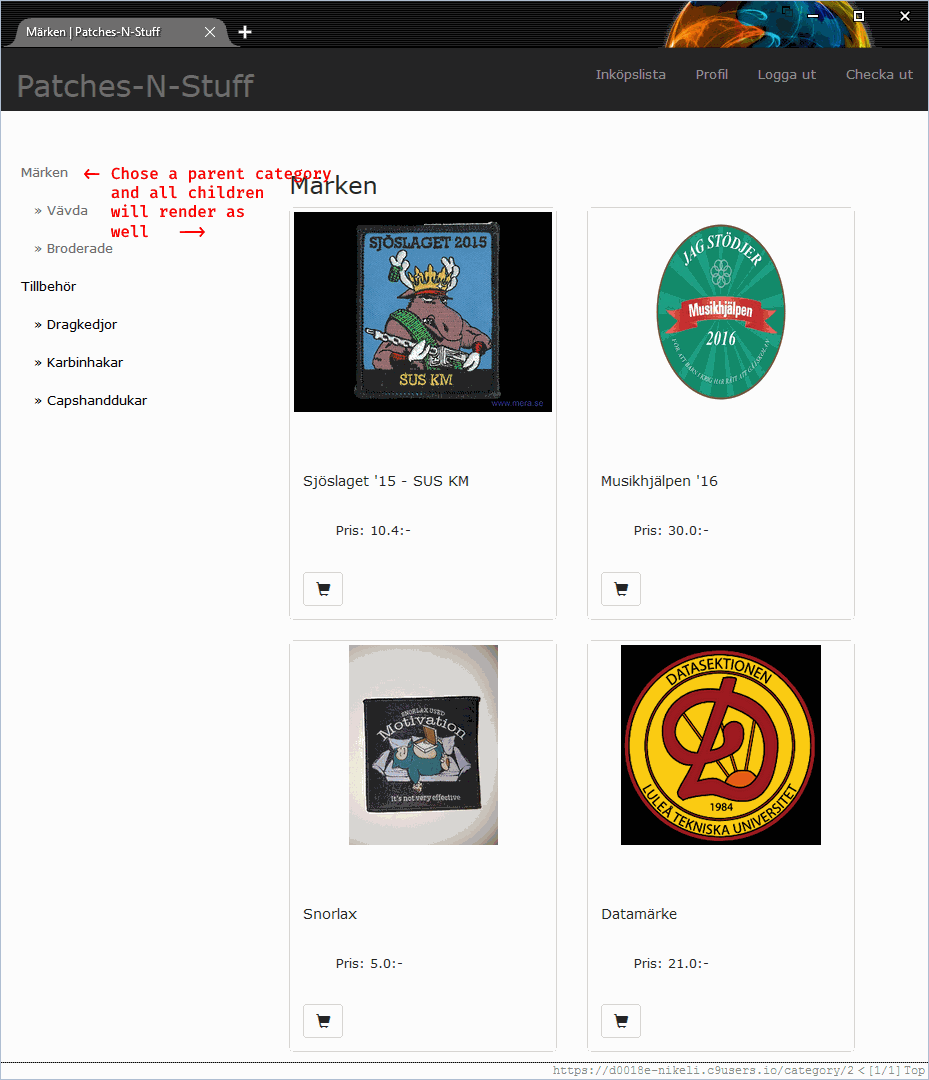
\includegraphics[width=0.9\paperwidth]{artifacts/stories/7_products.png}
	\caption{Category page}
	\label{fig:products}
\end{figure}

\begin{figure}
	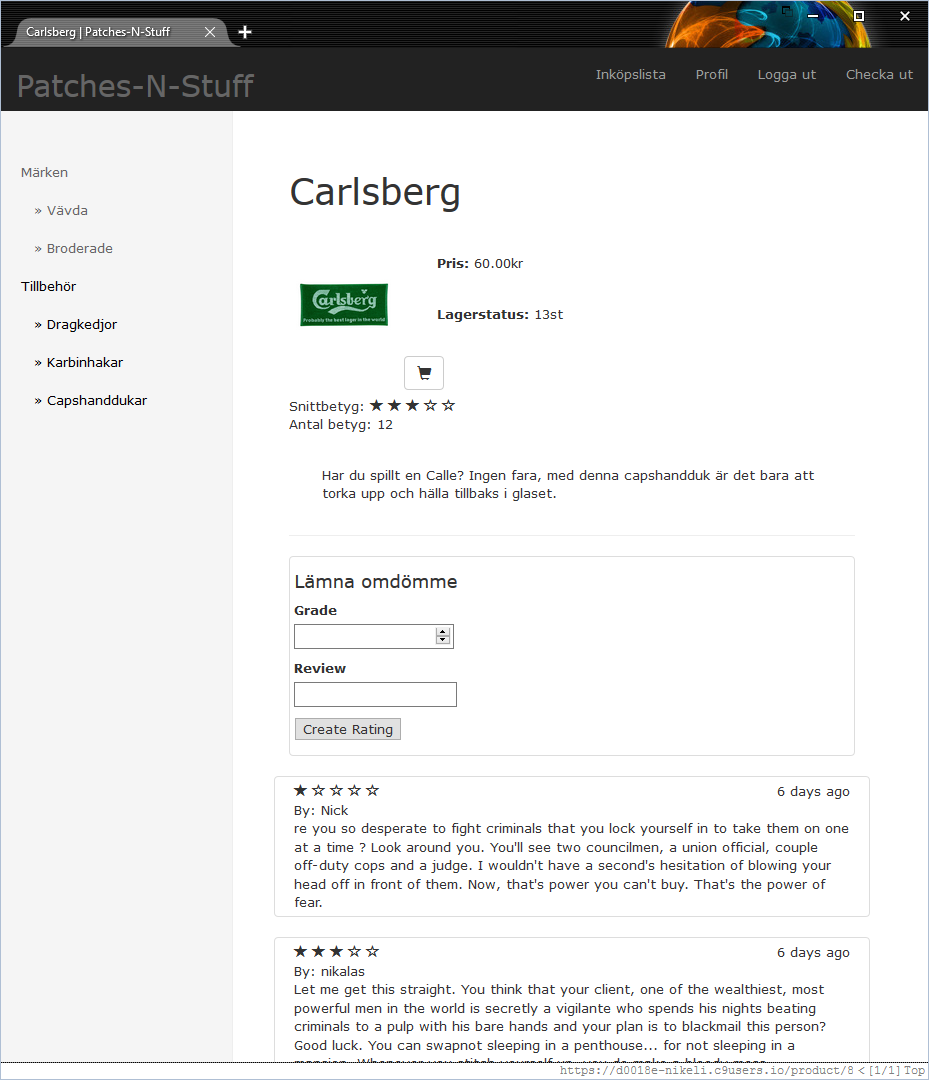
\includegraphics[width=0.9\paperwidth]{artifacts/stories/8_product.png}
	\caption{Product page}
	\label{fig:product}
\end{figure}

\begin{figure}
	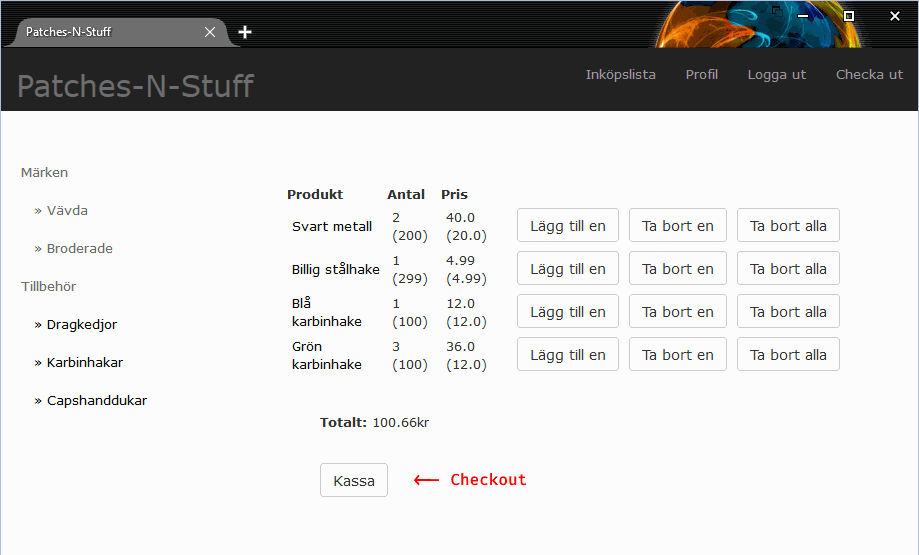
\includegraphics[width=0.9\paperwidth]{artifacts/stories/9_cart.png}
	\caption{Shopping cart}
	\label{fig:cart}
\end{figure}

\begin{figure}
	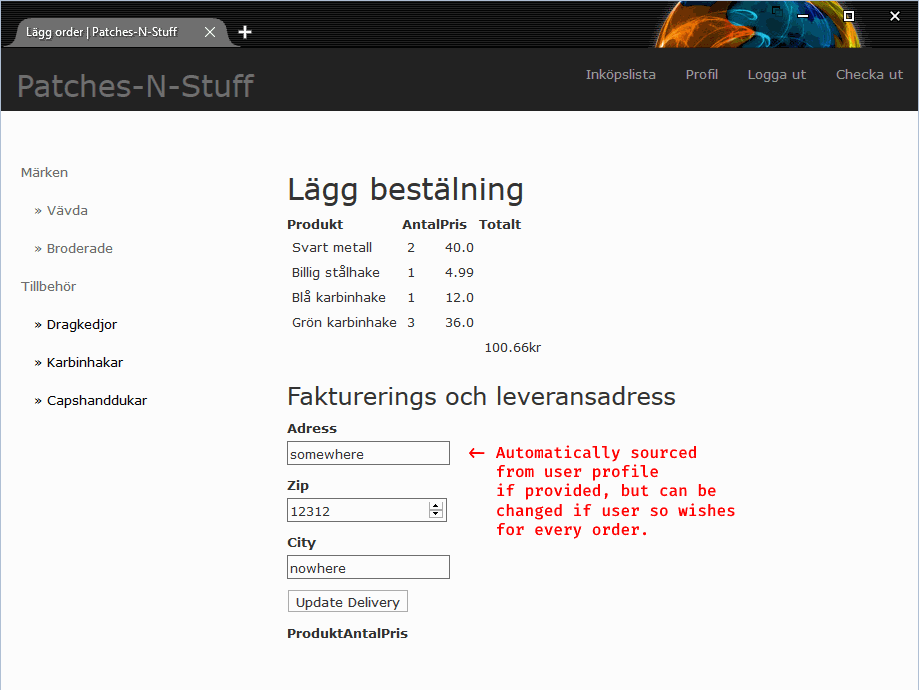
\includegraphics[width=0.9\paperwidth]{artifacts/stories/10_order.png}
	\caption{Order page}
	\label{fig:order}
\end{figure}

\begin{figure}
	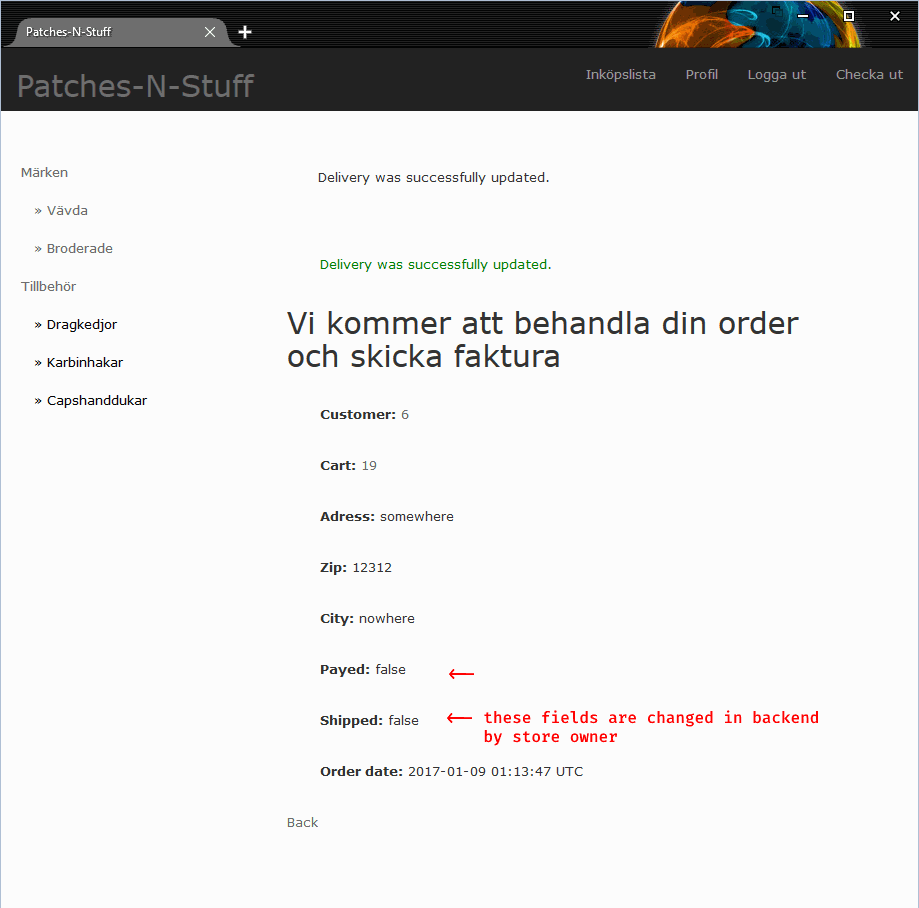
\includegraphics[width=0.9\paperwidth]{artifacts/stories/11_order_confirmation.png}
	\caption{Order confirmation}
	\label{fig:order_confirmation}
\end{figure}

\begin{figure}
	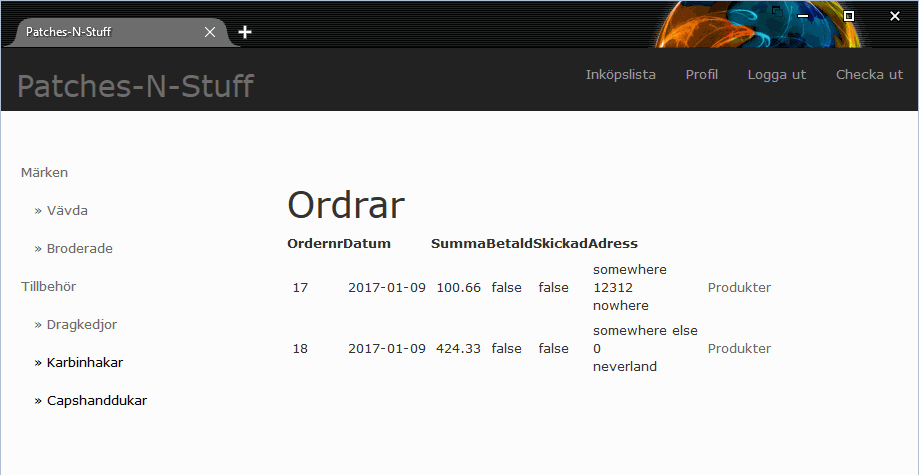
\includegraphics[width=0.9\paperwidth]{artifacts/stories/12_orders.png}
	\caption{Orders history}
	\label{fig:orders}
\end{figure}

\begin{figure}
	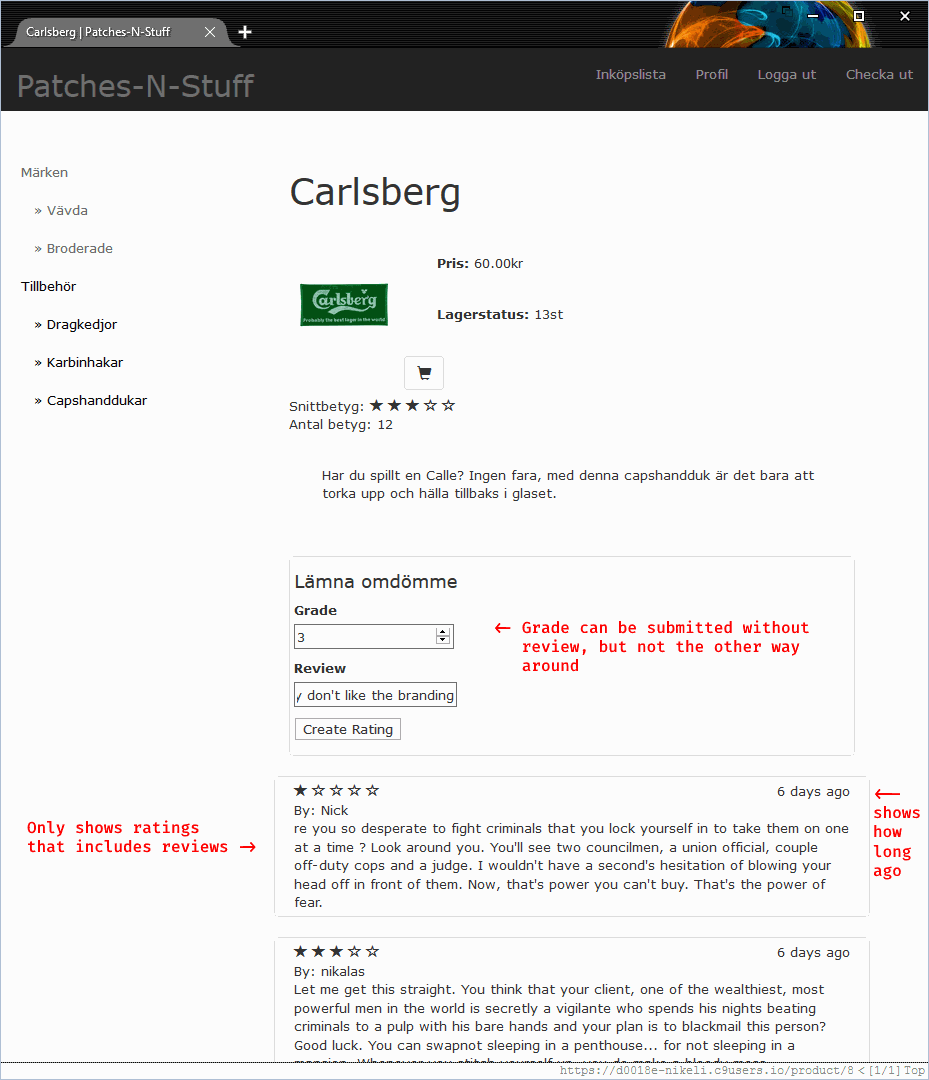
\includegraphics[width=0.9\paperwidth]{artifacts/stories/13_comments.png}
	\caption{User reviews}
	\label{fig:comments}
\end{figure}

\begin{figure}
	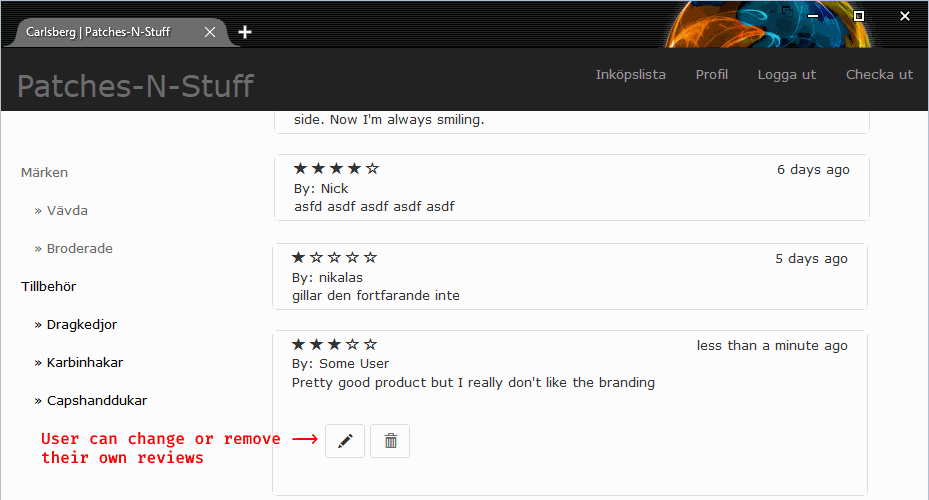
\includegraphics[width=0.9\paperwidth]{artifacts/stories/14_comment_added.png}
	\caption{Edit comment}
	\label{fig:comment_added}
\end{figure}

\begin{figure}
	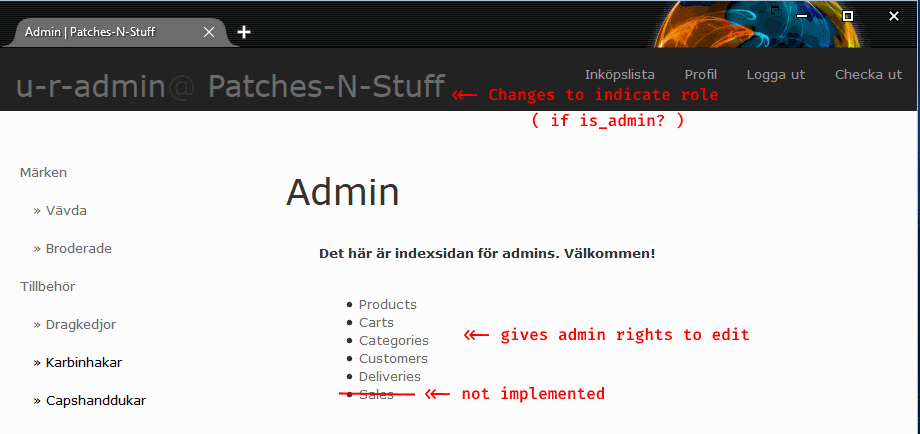
\includegraphics[width=0.9\paperwidth]{artifacts/stories/admin.png}
	\caption{Admin interface}
	\label{fig:admin}
\end{figure}
%TODO: Insert screen shots of whatever Miguel wanted us to add.

\end{document}
